% ОБЯЗАТЕЛЬНО ИМЕННО ТАКОЙ documentclass!
% (Основной кегль = 12pt, поэтому необходим extsizes)
% Формат, разумеется, А4
% article потому что стандарт не подразумевает разделов
% Глава = section, Параграф = subsection
% (понятия "глава" и "параграф" из стандарта)
\documentclass[a4paper, article, 12pt]{extarticle}

% Подключаем главный пакет со всем необходимым
\usepackage{spbudiploma}

% Пакет для русских букв в формулах
\usepackage{amsmath, amsfonts, amssymb, amsthm}

% Улучшаем обработку цитат
\usepackage{cite}

% Пакет для вставки картинок
\usepackage{graphicx}
\graphicspath{{images/}}
\DeclareGraphicsExtensions{.pdf, .png, .jpg}

% place pictuire exactly to the specified location
\usepackage{flafter}

% Пакет для подчеркивания текста
\usepackage{ulem}

% Добавляем ссылки в содержание
\usepackage[nottoc]{tocbibind}

% Вводим команду для символа нумерации
\newcommand*{\No}{\textnumero}

\begin{document}

\hyphenation{SPbU}

%\date{05.07.2020}

\begin{center}
	\Large{\textbf{Эссе на тему:}}\\
	\Large{\textbf{<<Исследование методов оценки трудоемкости алгоритма на основе эмпирического анализа>>}}\\
	\hfill \break
\end{center}

\tableofcontents

\section{Введение}\label{sec:introduction}

Оценка эффективности алгоритмов является важным этапом в создании качественных программных средств, причем один из критериев качества~--- временная эффективность, особенно актуальная для систем, работающих в режиме реального времени. Очевидно, что временная эффективность компьютерной программы связана с функцией трудоемкости алгоритма, т.\,е. с точным количеством операций, задаваемых алгоритмом в основе программной реализации. Однако, асимптотические оценки вычислительной сложности, получаемые в теоретическом исследовании алгоритмов, не всегда справедливы для конечного диапазона длин входов, что объясняется большими значениями коэффициентов у компонентов функции трудоемкости. В работе описывается практический подход на основе эмпирического анализа времени выполнения программной реализации.

Вычисление доверительной трудоемкости основано на построении доверительных интервалов оцениваемой величины трудоемкости с заданной доверительной вероятностью в классическом подходе математической статистики~\cite{petrushyn_ulyanov_analysis}. Преимущество упомянутого подхода заключается в использовании доверительной трудоемкости как гарантирующей оценки, повышающей точность результатов эмпирического анализа.

В данной работе проводится исследование применимости предложенного подхода на основе доверительной трудоемкости для большего количества алгоритмов и предлагается ряд улучшений для этого подхода.

\section{Постановка задачи}\label{sec:problem_statement}

Основными целями данной работы являются:

\begin{enumerate}
	\item[•] исследование применимости существующего подхода для более широкого класса алгоритмов;

	\item[•] выбор алгоритма для анализа;

	\item[•] вычисление доверительной трудоемкости алгоритма и сравнение полученных результатов с классическим эмпирическим подходом;

	\item[•] анализ полученных результатов.
\end{enumerate}

Исследование применимости состоит в ознакомлении с предложенным подходом и его адаптация для поддержки большего количества алгоритмов. В первую очередь стоит цель рассмотреть возможность применения альтернативных методов, не затронутых в работе~\cite{petrushyn_ulyanov_analysis}, на разных этапах анализа функции трудоемкости.

Для сравнения описанного подхода с классическим необходимо выбрать алгоритм для проведения анализа трудоемкости и применить модифицированный подход для вычисления функции трудоемкости.

\section{Описание подходов}\label{sec:review}

При разработке алгоритма для решения поставленной задачи всегда стоит вопрос о его корректности, для чего необходимо провести анализ алгоритма. Данный анализ включает в себя доказательство корректности или правильности алгоритма и установление его емкостных и временных характеристик, т.\,е. определение того, какое количество ресурсов требуется алгоритму для решения задачи. В данной работе рассматривается именно вторая часть анализа при начальном условии, что все рассматриваемые алгоритмы корректно решают поставленные задачи.

Одной из первых фундаментальных работ в области математического анализа сложности алгоритмов является~\cite{knuth}. Однако в ней, как и в других центральных работах по анализу алгоритмов~\cite{cormen, wegener} используются методы для вычисления трудоемкости алгоритма в среднем.

Совершенно новый подход был предложен в работе~\cite{petrushyn_ulyanov_analysis} для повышения точности результатов эмпирического анализа алгоритма. Для решения указанной задачи авторы рассматривают сложность алгоритма при заранее заданном и зафиксированном входном размере данных. Основная идея подхода состоит в построении доверительного интервала функции трудоемкости алгоритма. Для этого авторы используют бета"=распределение в качестве непрерывного распределения для аппроксимации значений трудоемкости. На практике данный подход показывает более реальные границы сложности алгоритма для рассматриваемых входных данных при заданном коэффициенте доверия.

\section{Исследование трудоемкости}\label{sec:complexity_research}

\subsection{Общие положения исследования}\label{sec:common_definitions}

Основной целью исследования является построение доверительной функции трудоемкости для рассматриваемого алгоритма. Стоит отметить, что объектом анализа выступает именно сам алгоритм, поскольку его программные реализации могут иметь совершенно разные показатели производительности на электронно"=вычислительных машинах. В дальнейшем будем использовать следующее общепринятое определение трудоемкости:

\Definition[n]{\,\,Трудоемкость алгоритма $A$ на входе $D$~--- количество базовых операций в заданной модели вычислений на рассматриваемом входе.}

Также введем обозначение $f_A(D)$ для функции трудоемкости алгоритма $A$ на входе $D$ и $D_n$ для совокупности всех входов $D$ размерности $n$. Предполагается, что закон распределения значений $f_A(D)$ неизвестен.

Теоретическое исследование трудоемкости имеет некоторые трудности при построении вероятностной модели для рассматриваемого алгоритма, такие как определение полной группы событий и определение вероятностной меры~\cite{petrushyn_ulyanov_definitions}. Поэтому разумным и единственным путем на данный момент остается экспериментальное исследование. В рамках такого исследования для функции трудоемкости вводится ограниченная дискретная случайная величина с неизвестным распределением и строится гистограмма относительных частот. Далее полученная гистограмма аппроксимируется некоторой функцией. Обычно аппроксимирующую функцию выбирают из множества хорошо изученных функций плотности распределения вероятностей.

Для доказательства того факта, что аппроксимация выбранной функцией плотности распределения является корректной, необходимо сформировать и доказать гипотезу о соответствующем распределении относительных частот значений функции трудоемкости~\cite{petrushyn_ulyanov_planning}. В случае, если гипотеза не будет доказана, необходимо выбрать другую функцию и повторить процедуру.

Основная проблема теоретических значений трудоемкости состоит в том, что полученные зависимости количества базовых операций от размеров входов могут быть не актуальны для подмножества входов алгоритма, которые используются в конкретных задачах на практике. Таким образом, актуальной становится проблема сокращения длины сегмента для оценки трудоемкости на рассматриваемом подмножестве входов.

Именно доверительная трудоемкость призвана решить описанную проблему~\cite{petrushyn_ulyanov_analysis}. Для выбранной аппроксимирующей функции распределения исследователями задается коэффициент доверия $\gamma$~\cite{koroluk}. После решения интегрального уравнения для рассматриваемой функции распределения можно получить значение $f_\gamma(n)$ трудоемкости, где $\gamma$~--- заданный коэффициент доверия. Данное значение называется доверительной трудоемкостью.

Одним из его важных свойств является то, что никакое другое значение функции трудоемкости не превысит доверительную трудоемкость для рассматриваемого единичного входа. В данном случае длина сегмента может быть существенно сокращена, поскольку для единичного входа алгоритма трудоемкость будет заключена в сегменте $[f^\vee, f_\gamma]$: между лучшим случаем и значением $f_\gamma(n)$ с вероятностью $\gamma$.

\subsection{Построение гистограммы частот}\label{sec:frequency_histogram}

Для построения гистограммы относительных частот по экспериментальным данным необходимо сперва нормировать данные. Введем случайную нормированную величину $T$. Ее реализации $t_i$ получаются на основе теоретических и эмпирических значений трудоемкости~\cite{petrushyn_ulyanov_analysis}:

\begin{equation}\label{eq:t_value}
	t_i = \frac{f_i - f^\vee}{f^\wedge - f^\vee},
\end{equation}

\noindent где $f_i$~--- значение трудоемкости для сгенерированных случайных допустимых входов $D_i$: $f_i = f_A(D_i), i = \overline{1, m}$, а $f^\wedge, f^\vee$~--- теоретический максимум и минимум функции трудоемкости соответственно. При этом отметим, что нормированные величины $t_i$ принимают значения из сегмента $[0, 1]$.

\subsection{Определение объема выборки}\label{sec:selection_size}

При построении гистограммы остался нерешенным вопрос о требуемом размере выборки. Стоит отметить, что в некоторых случаях исследователи имеют возможность работать только с ранее полученными выборками. Однако более распространены ситуации, когда возможность извлекать выборки есть. Даже в этом случае, очевидно, приоритет направлен в сторону минимизации объема выборок для эксперимента, что позволит уменьшить временные, ресурсные и финансовые затраты исследователей. Поэтому возникает проблема определения минимального числа экспериментов $m$ для вычисления трудоемкости алгоритма при заданной доверительной вероятности $\gamma$. Заметим, что длина входа $n$ при этом остается постоянной.

\subsubsection{Метод на основе закона распределения}\label{sec:distribution_selection_size}

Метод основан на рассмотрении гипотезы о законе распределения функции трудоемкости алгоритма~\cite{petrushyn_ulyanov_planning}. Поскольку закон распределения значений $f_A(D)$ неизвестен, вводится гипотеза, что значения функции трудоемкости являются ограниченной дискретной случайной величиной, которая распределена по одному из хорошо изученных законов распределения (примеры используемых законов распределения будут рассмотрены далее). Суть данного метода сводится к тому, что для определения минимального объема выборки $m$ проводятся ряд последовательных экспериментов с постоянной длиной входа $n$. Значение $n$ задается исследователями, как и начальный объем выборки $m$.

На каждой итерации извлекаются выборки размера $m$ и вычисляются значения трудоемкости. Далее рассчитывается ряд статистических величин: выборочное среднее $\overline{f_\text{э}}(m)$ и выборочная исправленная дисперсия $S^2$, которые являются оценками теоретической трудоемкости $\overline{f_A}$ и теоретической дисперсии трудоемкости $\sigma_A^2$ соответственно. Требуемый объем выборки рассчитывается по формуле:

\begin{equation}\label{eq:distribution_selection}
m^* = m^*(\delta, \gamma) = \min{m}: P(\abs*{\overline{f_\text{э}}(m) - \overline{f_A}} \leq \delta) \leq \gamma,
\end{equation}

\noindent т.\,е. минимальный объем выборки нужно выбирать таким образом, чтобы средние значения в выборке $\overline{f_\text{э}}$ позволяли построить доверительный интервал длиной $2\delta$, который покрывал бы неизвестное значение $\overline{f_A}$ с надежностью $\gamma$.

При этом условием останова для описанной последовательности итераций является выполнение неравенства:

\begin{equation}\label{eq:selection_size_stop}
m^*_\text{(i + 1)} < m^*_\text{(i)},
\end{equation}

\noindent где $m^*_\text{(i)}$~--- рассчитанный минимальный объем выборки на итерации $i$.

\subsection{Рассмотрение гипотезы о законе распределения}\label{sec:distribtuion_hypothesys}

При проведении анализа трудоемкости необходимо убедиться, что выбранный закон распределения соответствует наблюдаемым экспериментальным данным. В таком случае необходимо сформировать, рассмотреть и принять или отвергнуть гипотезу о соответствующем законе распределения.

Рассмотрим несколько широко применяемых критериев проверки статистических гипотез.

\subsubsection{Критерий согласия Пирсона ($\chi^2$)}\label{sec:pirson_criteria}

Критерий Пирсона проверяет значимость расхождения теоретической плотностью и эмпирической гистограммы относительных частот. В качестве нулевой гипотезы $H_0$ выступает предположение о соответствии выбранного теоретического закона распределения реальным результатам экспериментов. Заметим, что гипотеза $H_0$ является сложной, поскольку рассматривается закон распределения с восстановленными по выборке параметрами. Тогда критерий $\chi^2$ вычисляется по формуле~\cite{koroluk}:

\begin{equation}\label{eq:pirson_criteria}
	\chi_m^2 = m \cdot \sum_{i=1}^{k}{\frac{O_i - E_i}{E_i}},
\end{equation}

\noindent где $O_i, E_i$~--- относительные эмпирические и теоретические частоты в $i$"=ом сегменте гистограммы соответственно, $m$~--- общий размер выборки, $k$~--- количество полусегментов гистограммы. Величина $\chi_m^2$ имеет закон распределения $\chi^2$ с $s$ степенями свободы ($s = k - 1 - r$, где $r$~--- число параметров выбранного распределения).

Рассчитанное по формуле~\eqref{eq:pirson_criteria} значение сравнивается со значением правосторонней критической области:

\begin{equation}\label{eq:pirson_criteria_test}
	\chi_m^2 < \chi_\text{кр}^2(\alpha^{'}, s),
\end{equation}

\noindent где $\alpha^{'}$~--- заданный уровень значимости, $s$~--- количество степеней свободы, а значение $\chi_\text{кр}^2(\alpha^{'}, s)$ определяется по теоретическому распределению $\chi_m^2$. Гипотеза $H_0$ принимается, если выполняется неравенство~\eqref{eq:pirson_criteria_test}. В противном случае $H_0$ отвергается, необходимо выбрать другой закон распределения, построить соответствующую гистограмму относительных частот и снова рассмотреть гипотезу о законе распределения.

Отметим, что критерий Пирсона является состоятельным, т.\,е. почти наверняка отвергает ошибочную гипотезу при достаточно большом количестве испытаний. Также данный критерий обеспечивает минимальную возможную ошибку второго рода по сравнению с другими критериями~\cite{petrushyn_ulyanov_definitions}. Рекомендуется использовать критерий $\chi^2$ при достаточно большом размере выборки ($m > 100$) и количестве наблюдений в отдельном сегменте гистограммы относительных частот более 10~\cite{koroluk}. Если в какой"=либо сегмент попадает менее 10 значений выборки, необходимо объединить его с ближайшим. Иначе следует использовать другие критерии проверки статистических гипотез.

\subsubsection{Критерий согласия Колмогорова}\label{sec:kolmogorov_criteria}

Критерий Колмогорова проверяет значимость расхождения эмпирической и теоретической функций распределения. Нулевая гипотеза $H_0$ выбирается так же, как и при рассмотрении критерии Пирсона. Тогда критерий Колмогорова вычисляется по формуле~\cite{koroluk}:

\begin{equation}\label{eq:kolmogorov_criteria}
	D_m = \sup_{\abs*{x} < \infty}{\abs*{F_m(x) - F(x, \theta)}},
\end{equation}

\noindent где $F_m(x)$~--- эмпирическая функция распределения, $F(x, \theta)$~--- теоретическая функция распределения.

По теореме Колмогорова~\cite{koroluk} при справедливости проверяемой гипотезы:

\begin{equation}\label{eq:kolmogorov_test}
	\forall z > 0: \lim_{n \rightarrow \infty}{P\{\sqrt{m} \cdot D_m < z\}} = K(z) = \sum_{j = -\infty}^{+\infty}{(-1)^j \cdot e^{-2 \cdot j^2 \cdot z^2}}.
\end{equation}

\noindent Гипотеза $H_0$ принимается, если значение $\sqrt{m} \cdot D_m$ не превышает квантиль распределения $K_{\alpha^{'}}$, где $\alpha^{'}$~--- заданный уровень значимости.

Классический критерий Колмогорова стоит применять только для простых гипотез. При применении данного критерия для сложных гипотез появляются определенные различия, которые необходимо учитывать отдельно~\cite{kac}.

\subsection{Прогнозирование функции трудоемкости}\label{sec:compelixy_prediction}

Получение значений доверительной трудоемкости $f_{\gamma}(n)$ на интересующем исследователей сегменте требует значительных вычислительных затрат. Это обусловлено применением одного из методов восстановления параметров аппроксимирующего распределения на основе экспериментальных данных. Для решения проблемы сокращения временных затрат можно попытаться спрогнозировать выборочную дисперсию и выборочную среднюю с помощью функций регрессии. Уравнения регрессии могут быть построены на основе анализа имеющихся данных из меньшего сегмента входных данных. Таким образом, это позволит экстраполировать значения доверительной трудоемкости $f_{\gamma}(n)$ на весь интересующий сегмент, не проводя дополнительных экспериментов.

Обычно строят несколько функций регрессии, затем выбирают наилучшую из них. Набор функций для рассмотрения зависит от конкретной задачи и определяется оценкой имеющихся данных. Для задачи прогнозирования трудоемкости выбор функции регрессии можно осуществить одним из методов регрессионного анализа. Далее будет использоваться метод наименьших квадратов~\cite{hughes}. Сравнение функций разного вида будет производиться по коэффициенту детерминации $R^2$~\cite{hughes}.

Коэффициент детерминации является одним из наиболее используемых критериев оценки качества линейных и нелинейных моделей. Данный коэффициент следует применять с осторожностью, поскольку его значение увеличивается от добавления в модель новых переменных, даже в случаях, когда новые переменные не оказывают никакого влияния на объясняемую переменную.

\section{Проведение экспериментального исследования трудоемкости}\label{sec:practical_complexity_research}

\subsection{Описание выбранного алгоритма}\label{sec:pallotino_algorithm}

Нахождение кратчайшего пути от одной вершины до всех остальных является одной из основных задач оптимизации сети. Существует несколько распространенных и хорошо известных алгоритмов, которые решают эту проблему. Основные категории состоят из алгоритма Дейкстры и его модификаций, а также из алгоритма Беллмана\,--\,Форда\,--\,Мура и его модификаций. Есть также ряд других алгоритмов, которые не входят в эти категории.

Алгоритм Паллоттино~\cite{pallottino}~--- алгоритм, который находит кратчайшее расстояние от одной из вершин до всех остальных на графах без петель, является модификацией алгоритма Беллмана\,--\,Форда\,--\,Мура. Алгоритм Паллоттино применим для графов с ребрами отрицательного веса при отсутствии отрицательных циклов. Он широко используется для решения задач оптимального распределения грузопотоков по транспортной сети и выбора наиболее выгодных путей ее развития.

Входными данными для алгоритма является граф $G$, представленный в виде упорядоченной совокупности множеств вершин $V$ и ребер $E$: $G = (V, E)$. Оценка размера входных данных производится по размеру множеств вершин и ребер. Пусть $n$~--- количество вершин в множестве $V$, $l$~--- количество ребер в множестве $E$: $n = |V|, l = |E|$. В качестве базовой операции алгоритма выберем операцию релаксации ребра.

Алгоритм и генератор графов были реализованы на языке программирования C++. Результаты замеров анализировались в пакете Microsoft Excel. Для анализа алгоритма Паллоттино был использован генератор полных графов без мультиребер. Стоит отметить, что генератор входных данных должен обеспечивать репрезентативность выборки, т.\,е. генерировать такие входные данные, которые соответствуют особенностям применения алгоритма. Поскольку алгоритм Паллоттино используется для решения транспортных задач, в реализацию генератора было добавлено условие: для любых трех узлов графа должно выполняться неравенство треугольника. Пусть $G = (V, E)$~--- полный неориентированный граф с $n$ вершинами, $W: E \rightarrow R_+$~--- функция весов ребер. Тогда неравенство треугольника имеет вид:

\begin{equation}\label{eq:triangle_inequality}
	W((u, w)) \leq W((v, u)) + W((u, w)), \forall u, v, w \in V.
\end{equation}

Отметим, что алгоритм Паллоттино имеет оценки

\begin{equation}\label{eq:pallottino_best}
	O(n, l) = n,
\end{equation}

\begin{equation}\label{eq:pallottino_average}
	O(n, l) = n \cdot l,
\end{equation}

\begin{equation}\label{eq:pallottino_worst}
	O(n, l) = n^2 \cdot l
\end{equation}

в лучшем, среднем и худшем случаях соответственно~\cite{pallottino}.

\subsection{Этап предварительного исследования}\label{sec:analysis_part_1}

\subsubsection{Основные шаги}\label{subsec:analysis_part_1_intro}

Поскольку организация экспериментального исследования сложности алгоритма требует подсчета выполняемых основных операций на полученном входе, в исходный код реализации алгоритма Паллоттино были добавлены счетчики. По результатам каждого эксперимента программная реализация алгоритма сохраняет число основных операций в файл для дальнейшей обработки.

Рассмотрим более подробно этап планирования предварительного исследования~\cite{petrushyn_ulyanov_planning}. Основная задача этого этапа~--- определение необходимого размера выборки при фиксированной длине входа для проведения основного этапа исследований.

Выдвигается гипотеза, что функция трудоемкости алгоритма Паллоттино имеет бета"=распределение. Бета"=распределение отличается большой универсальностью поведения. Плотность вероятности является очень гибкой за счет своих параметров $\alpha$ и $\beta$, что позволяет получать другие распределения (например, равномерное распределение). Аналогичного результата можно добиться, комбинируя несколько бета"=распределений с разными значениями параметров (например, треугольное распределение)~\cite{petrushyn_ulyanov_definitions}. Основные шаги предварительного исследования:

\begin{enumerate}
	\item Фиксация некоторого значения длины входа $n$ из сегмента длин в области применения алгоритма Паллоттино. В рассматриваемом случае $n = 80$.

	\item Определение необходимого числа экспериментов $m$ (объем выборки) с программной реализацией алгоритма одним из описанных ранее способов.

	\item Проведение экспериментального исследования и получение значений трудоемкости $f_i$ для сгенерированных случайных допустимых входов $D_i$: $f_i = f_A(D_i), i = \overline{1, m}$.

	\item Получение теоретических функций трудоемкости алгоритма для лучшего и худшего случаев. Функции $f_A^\vee$ и $f_A^\wedge$ для алгоритма Паллоттино имеют вид:

	\begin{equation}\label{eq:complexity_function_1}
		f_A^\vee(n) = n,
	\end{equation}

	\begin{equation}\label{eq:complexity_function_2}
		f_A^\wedge(n) = \frac{n^3 \cdot (n - 1)}{2}.
	\end{equation}

	Последняя формула следует из того, что алгоритм Паллоттино в худшем случае имеет оценку~\eqref{eq:pallottino_worst}, а поскольку для полных графов\\$l = {n \cdot (n - 1) \over{2}}$, получаем~\eqref{eq:complexity_function_2}.

	\item Выбор числа $k$ полусегментов для гистограммы относительных частот значений трудоемкости.

	\item Нормирование значений трудоемкости, полученной путем проведения экспериментального исследования, и построение на основе нормированных данных гистограммы относительных частот.

	\item Вычисление нормированного выборочного среднего и нормированной исправленной выборочной дисперсии по формулам~\cite{petrushyn_ulyanov_planning}:

	\begin{equation}\label{eq:mean}
		\overline{t} = \frac{\overline{f_t}(n) - f^\wedge}{f^\wedge - f^\vee},
	\end{equation}

	\begin{equation}\label{eq:variance}
		s^2 = \frac{1}{m - 1} \sum_{i=1}^{m}{\frac{(f_i - \overline{f_t}(n))^2}{(f^\wedge - f^\vee)^2}},
	\end{equation}

	где $f^\wedge$ и $f^\vee$~--- соответственно максимальное и минимальное значение теоретических функций трудоемкости, $\overline{f_t}(n)$~--- выборочное среднее.
	
	\item Формулировка гипотезы об аппроксимирующем законе распределения и расчет параметров этого закона. В рассматриваемом случае выдвигается гипотеза о бета"=распределении. Параметры бета"=распределения рассчитываются по формулам~\cite{petrushyn_ulyanov_planning}:

	\begin{equation}\label{eq:alpha}
		\alpha = \frac{\overline{t}}{s^2} (\overline{t} - (\overline{t})^2 - s^2),
	\end{equation}

	\begin{equation}\label{eq:beta}
		\beta = \frac{(1 - \overline{t})}{s^2} (\overline{t} - (\overline{t})^2 - s^2).
	\end{equation}

	\item Расчет теоретических частот по формуле функции плотности~\cite{petrushyn_ulyanov_planning}:

	\begin{equation}\label{eq:frequency}
		p_i = \int_{x_i}^{x_i + \Delta x_i}{b(x, \alpha, \beta) dx},
	\end{equation}

	где $b$~--- функция бета"=распределения.

	\item Расчет наблюдаемого значения критерия согласия Пирсона по формуле~\cite{koroluk}:
	
	\begin{equation}\label{eq:pirson_criteria_concrete}
		\chi_{\text{набл}}^2 = m \sum_{i=1}^{s} \frac{(w_i - p_i)^2}{p_i},
	\end{equation}

	где $w_i$~--- относительные частоты.

	\item Проверка гипотезы о законе распределения: если нулевая гипотеза принимается, то переход к основному этапу исследования. Иначе~--- выбор другого закона распределения и повтор шагов 8--11.
\end{enumerate}

\subsubsection{Результаты предварительного исследования}\label{subsec:results_part_1}

Для оценки необходимого числа экспериментов с программной реализацией алгоритма Паллоттино для фиксированной длины входа ($n = 80$) в соответствии с описанной методикой был проведен этап предварительного исследования с коэффициентом доверия $\gamma = 0.95$ и относительной ошибкой $\varepsilon = 0.001$. Для определения необходимого числа экспериментов использовался метод на основе бета"=распределения~\cite{petrushyn_ulyanov_planning}. Суть метода была изложена ранее.

Сначала была извлечена выборка объемом 200, вычислено значение $m_{(1)}^*$, результаты расчетов приведены в таблице 1.

\begin{center}\label{table1}
	\begin{small}
		\textbf{Таблица 1.}
	\end{small}\\
	\hfill \break
	\begin{tabular}{|c|c|}
		\hline
		Предварительный объем выборки & 200\\
		\hline
		Выборочное среднее & 9372.87\\
		\hline
		Выборочная дисперсия & 2774677.39005\\
		\hline
		Нормированное среднее & 0.000459499\\
		\hline
		Нормированная дисперсия & 0.000000006784\\
		\hline
		Альфа & 31.10865322\\
		\hline
		Бета & 67670.14123\\
		\hline
		Дельта для $\varepsilon = 0.001$ & 9.401506539\\
		\hline
		Нижний предел интегрирования & 0.000459034\\
		\hline
		Верхний предел интегрирования & 0.000459964\\
		\hline
		Рассчитанный объем выборки & 84934\\
		\hline
	\end{tabular}
\end{center}

Далее была извлечена выборка объемом 84934, результаты расчетов приведены в таблице 2. Полученный объем выборки оказался меньше, чем объем выборки текущего эксперимента, поэтому необходимое количество экспериментов $m = 104435$.

\begin{center}\label{table4}
	\begin{small}
		\textbf{Таблица 2.}
	\end{small}\\
	\hfill \break
	\begin{tabular}{|c|c|}
		\hline
		Предварительный объем выборки & 84934\\
		\hline
		Выборочное среднее & 9526.48\\
		\hline
		Выборочная дисперсия & 3524490.40991\\
		\hline
		Нормированное среднее & 0.000467095\\
		\hline
		Нормированная дисперсия & 0.000000008617\\
		\hline
		Альфа & 25.30655136\\
		\hline
		Бета & 54153.34542\\
		\hline
		Дельта для $\varepsilon = 0.001$ & 7.983101972\\
		\hline
		Нижний предел интегрирования & 0.0004667\\
		\hline
		Верхний предел интегрирования & 0.000467489\\
		\hline
		Рассчитанный объем выборки & 104435\\
		\hline
	\end{tabular}
\end{center}

Далее была извлечена итоговая выборка объемом 104435 и построена гистограмма относительных частот на 387 полусегментах с помощью пакета Microsoft Excel. Далее произведено нормирование значений экспериментальной трудоемкости. На основе полученных данных построена гистограмма относительных частот, она представлена на рис.~\ref{fig:histogram}. Значения параметров бета"=распределения для итоговой выборки: $\alpha = 25.24821, \beta = 53988.69414$.

\begin{figure}[h]
	\center{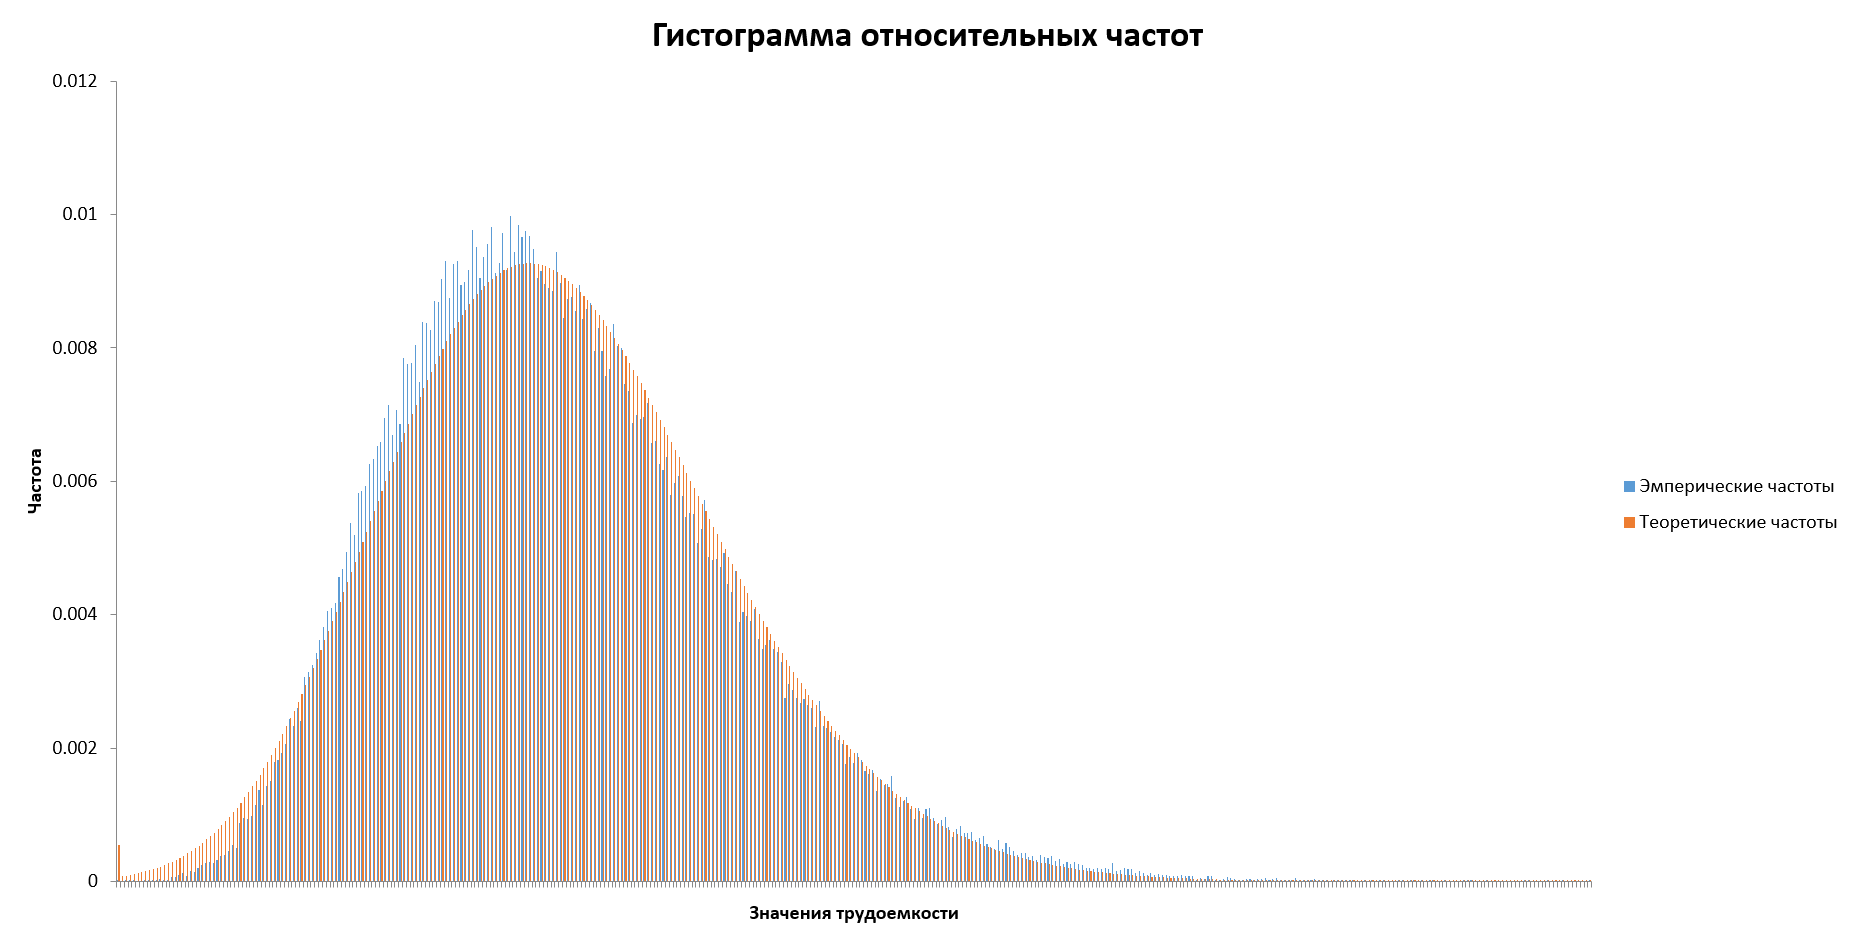
\includegraphics[width=\linewidth]{histogram.png}}
	\caption{Теоретические и эмпирические частоты для алгоритма Паллоттино при $n = 80$ с разбиением нормированного сегмента [0, 1] на 387 полусегментов}
	\label{fig:histogram}
\end{figure}

Результаты расчетов теоретических частот по функции плотности приведены на рис.~\ref{fig:histogram}. Наблюдаемое значения критерия Пирсона в данном случае $\chi_{\text{набл}}^2 = 282.24386$. Поскольку $\chi_{\text{кр}}^2(0.05, 384) = 430.69192$ (вычислено стандартной функцией пакета Microsoft Excel), получаем $\chi_{\text{набл}}^2 < \chi_{\text{кр}}^2(0.05, 384)$. Следовательно, нет оснований отвергать нулевую гипотезу и можно перейти к основному этапу исследования.

\subsection{Этап основного исследования}\label{sec:analysis_part_2}

\subsubsection{Основные шаги}\label{subsec:analysis_part_2_intro}

Основная задача этапа основного исследования~--- построение функции доверительной трудоемкости на основе данных, полученных из экспериментального исследования.

\begin{enumerate}
	\item Определение первого сегмента значений длин входа. Выбор производится исследователем в соответствии с особенностями применения алгоритма. В рассматриваемом случае алгоритма Паллоттино будет применяться для графов с количеством вершин от 80 до 2560;

	\item Определение второго сегмента значений длин входа. Данный сегмент будет использоваться для проведения экспериментального исследования. В рассматриваемом примере таким сегментом является сегмент от 80 до 320;

	\item Выбор шага изменения длины входа для второго сегмента. Данный шаг будет использоваться для проведения экспериментального исследования. В рассматриваемом случае значение шага равно 10;

	\item Определение необходимого числа $m$ экспериментов с программной реализацией алгоритма для фиксированной длины входа. По итогам экспериментального исследования определяется выборочная средняя и дисперсия. В данном случае по результатам предварительного этапа исследования $m = 104435$;

	\item Расчет на основе данных, полученных из экспериментального исследования, выборочной средней и дисперсии для каждого значения $n$. В рассматриваемом случае $n$ изменяется от 80 до 320 с шагом 10;

	\item Проведение анализа для экспериментальных данных. На данном шаге строится уравнение регрессии для выборочной средней и дисперсии;

	\item Расчет на основе результатов, полученных на шаге 5, параметров аппроксимирующего бета"=распределения по формулам~\eqref{eq:alpha},~\eqref{eq:beta} как функций длины входа $\alpha(n), \beta(n)$;

	\item Определение значения коэффициента доверия и вычисление значений левого $\gamma$"=квантиля бета"=распределения~\cite{petrushyn_ulyanov_definitions}: $x_\gamma(n) = B^{-1}(\gamma, \alpha(n), \beta(n))$;

	\item Вычисление значений функции доверительной трудоемкости для исследуемого сегмента длин входа по формуле~\cite{petrushyn_ulyanov_analysis}:

	\begin{equation}\label{eq:final_complexity_fucntion}
		f_\gamma(n) = f^\vee(n) + x_\gamma(n) (f^\wedge(n) - f^\vee(n)).
	\end{equation}
\end{enumerate}

\subsubsection{Результаты основного исследования}\label{subsec:results_part_2}

Было проведено основное исследование с выборками объемом 104435 для входных данных в сегменте $n = [80, 2560]$. Для полученных результатов построены уравнения регрессии для нормированной выборочной средней и выборочной дисперсии. В первом случае уравнение регрессии имеет вид $\overline{t} = 0.9449 \cdot n^{-1.1735}$, во втором~--- $s^2 = y = 0.1165 \cdot n^{-3.741}$. В данном случае $y = ax^{-b}$~--- наилучший в смысле максимума значения коэффициента детерминации $R^2$ вид функции, подбор коэффициентов осуществлен с помощью метода наименьших квадратов (расчеты выполнены в Microsoft Excel).

\begin{figure}[h]
	\center{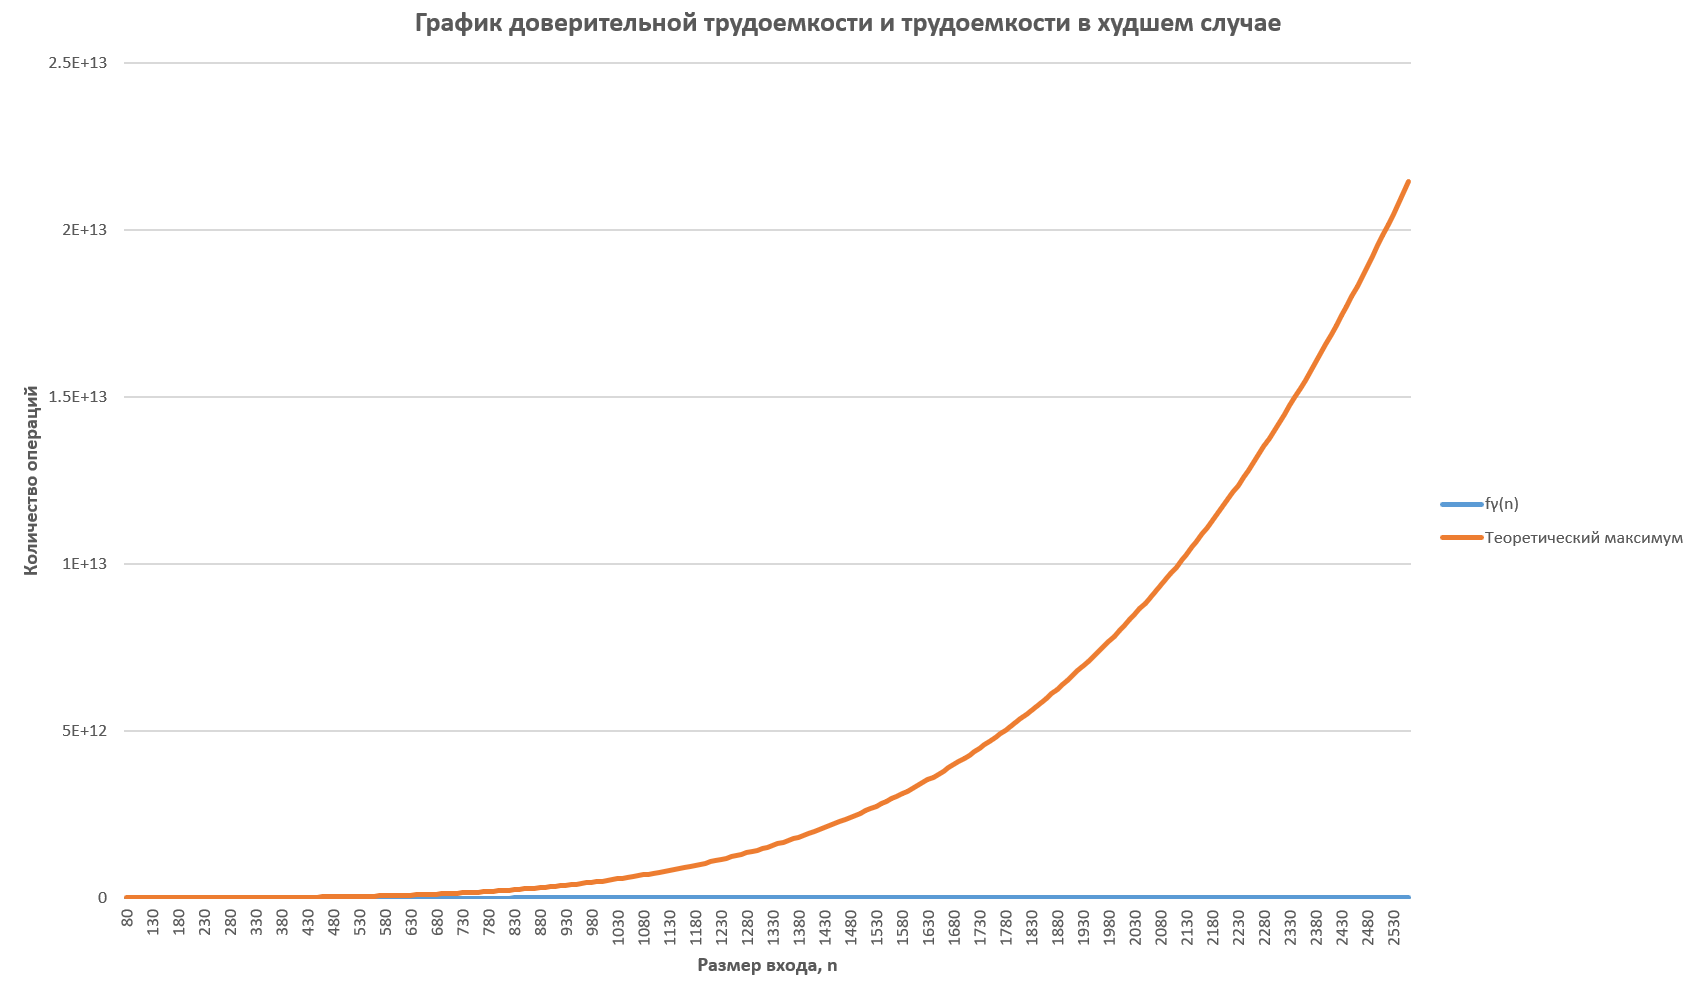
\includegraphics[width=\linewidth]{comparison.png}}
	\caption{График доверительной трудоемкости и трудоемкости в худшем случае для алгоритма Паллоттино}
	\label{fig:comparison_complexities}
\end{figure}

В рассматриваемом примере $\gamma = 0.95, \alpha < \beta$. На рис.~\ref{fig:comparison_complexities} показан график значений доверительной трудоемкости и трудоемкости в худшем случае для алгоритма Паллоттино на сегменте $n = [80, 2560]$. Отдельно стоит отметить, что доверительная трудоемкость получена для значения коэффициента доверия $\gamma = 0.95$, т.~е. в 95\% случаев наблюдаемая в единичном эксперименте трудоемкость алгоритма не будет превышать значение доверительной трудоемкости. Для рассматриваемого алгоритма Паллоттино эти значения в несколько раз меньше трудоемкости в худшем случае на исследуемом сегменте длин входа.

\section{Заключение}\label{sec:summary}

Исследованы различные дополнительные методы для применения методологии~\cite{petrushyn_ulyanov_analysis} для более широкого класса алгоритмов.

Эксперимент с алгоритмом Паллоттино показал, что оценка функции сложности в худшем случае может приводить к существенному завышению временного прогноза из"=за малой вероятности входных данных, обеспечивающих максимум функции трудоемкости для рассматриваемой задачи. Полученные результаты подтверждают возможность повышения достоверности прогнозирования временной эффективности компьютерных алгоритмов и более эффективного решения задачи выбора рациональных алгоритмов на основе сравнительного анализа функций доверительной трудоемкости вместо традиционного сравнения трудоемкости в среднем случае.

% Библиография в CPS Conf стиле.
% Аргумент {1} ниже включает переопределенный стиль с выравниванием слева.
%\section{Список литературы}\label{sec:sources}
\begin{thebibliography}{1}\label{sec:sources}
	% №1
	\bibitem{petrushyn_ulyanov_analysis} Петрушин~В.\:Н., Ульянов~М.\:В., Кривенцов~А.\:С. Доверительная трудоемкость~--- новая оценка качества алгоритмов // Информационные технологии и вычислительные системы. 2009. \No~2. С.~23--37.

	% №2
	\bibitem{knuth} Knuth~D. The Art of Computer Programming / Addison\,--\,Wesley, 1968.

	% №3
	\bibitem{cormen} Cormen~T.\:H., Leiserson~C.\:E., Rivest~R.\:L., Stein~C. Introduction to Algorithms. Chapter 1: Foundations (Second ed.) // Cambridge, MA: MIT Press and McGraw-Hill. 2001. P.~3--122.

	% №4
	\bibitem{wegener} Wegener~I. Complexity theory: exploring the limits of efficient algorithms // Berlin, New York: Springer\,--\,Verlag. P.~20.

	% №5
	\bibitem{petrushyn_ulyanov_definitions} Петрушин~В.\:Н., Ульянов~М.\:В. Информационная чувствительность компьютерных алгоритмов. М.: Физматлит, 2010.

	% №6
	\bibitem{petrushyn_ulyanov_planning} Петрушин~В.\:Н., Ульянов~М.\:В. Планирование экспериментального исследования трудоемкости алгоритмов на основе бета"=распределения // Информационные технологии и вычислительные системы. 2008. \No~2. С.~81--91.

	% №7
	\bibitem{koroluk} Королюк~В.\:С., Портенко~Н.\:И., Скороход~А.\:В., Турбин~А.\:Ф. Справочник по теории вероятностей и математической статистике. М.: Наука, 1985.

	% №8
	\bibitem{kac} Kac~M., Kiefer~J., Wolfowitz~J. On Tests of Normality and Other Tests of Goodness of Fit Based on Distance Methods // Ann. Math. Stat., 1955. Vol.~26. P.~189--211.

	% №9
	\bibitem{hughes} Hughes~A., Grawoig~D. Statistics: A Foundation for Analysis / Addison\,--\,Wesley, 1971.

	% №10
	\bibitem{pallottino} Pallottino~S. Shortest"=path methods: Complexity, interrelations and new propositions // Networks. 1984. Vol.~14. P.~257--267.

\end{thebibliography}

\end{document}
